% ============================================================
% REPORTE TÉCNICO — Clasificación Médica Multimodal con MoE
% Incorporar Elementos de IA (Bloque Visión)
% Formato: IEEE/ABET | Máx. 7 páginas | Times New Roman 11pt
% ============================================================

\documentclass[11pt, a4paper]{article}

% ─── Paquetes ────────────────────────────────────────────────
\usepackage[utf8]{inputenc}
\usepackage[T1]{fontenc}
\usepackage[spanish]{babel}
\usepackage{times}                      % Times New Roman
\usepackage[top=2.5cm, bottom=2.5cm,
            left=2.5cm, right=2.5cm]{geometry}
\usepackage{setspace}                   % Interlineado
\usepackage{booktabs}                   % Tablas profesionales
\usepackage{graphicx}
\graphicspath{{checkpoints/figures/}{./}}
\usepackage{amsmath}
\usepackage{hyperref}
\usepackage{caption}
\usepackage{subcaption}
\usepackage{float}
\usepackage{multirow}
\usepackage{array}
\usepackage{xcolor}
\usepackage{enumitem}
\usepackage{titlesec}
\usepackage{fancyhdr}
\usepackage[numbers]{natbib}
\usepackage{tikz}
\usetikzlibrary{arrows.meta, positioning, shapes.geometric, fit, backgrounds}

% ─── Configuración global ────────────────────────────────────
\setstretch{1.15}
\setlength{\parskip}{2pt}
\setlength{\parindent}{0pt}

\titleformat{\section}{\normalfont\bfseries\normalsize}{\thesection.}{0.5em}{}
\titleformat{\subsection}{\normalfont\bfseries\small}{\thesubsection.}{0.5em}{}
\titlespacing*{\section}{0pt}{4pt}{2pt}
\titlespacing*{\subsection}{0pt}{3pt}{1pt}

% Reduce float spacing
\setlength{\textfloatsep}{6pt plus 1pt minus 1pt}
\setlength{\floatsep}{6pt plus 1pt minus 1pt}
\setlength{\intextsep}{6pt plus 1pt minus 1pt}
\setlength{\abovecaptionskip}{3pt}
\setlength{\belowcaptionskip}{0pt}

\captionsetup{font=small, labelfont=bf}

\pagestyle{fancy}
\fancyhf{}
\rhead{\small Clasificación Médica con MoE}
\lhead{\small UAO — Analítica de Datos}
\cfoot{\thepage}
\renewcommand{\headrulewidth}{0.4pt}

\hypersetup{colorlinks=true, linkcolor=black, citecolor=black, urlcolor=blue}

% ============================================================
\begin{document}
% ============================================================

% ─── PORTADA ─────────────────────────────────────────────────
\begin{titlepage}
\centering
\vspace*{1cm}
{\large \textbf{Universidad Autónoma de Occidente}}\\[0.3cm]
{\normalsize Facultad de Ingeniería — Ingeniería de Datos e Inteligencia Artificial}\\[0.3cm]

\rule{\linewidth}{1pt}\\[0.4cm]
{\LARGE \textbf{Clasificación Médica Multimodal}}\\[0.2cm]
{\Large \textbf{con Mixture of Experts y Ablation Study del Router}}\\[0.4cm]
\rule{\linewidth}{1pt}\\[1.5cm]

{\normalsize
\begin{tabular}{ll}
\textbf{Estudiantes:} & Sebastián Belalcazar Mosquera \\
                      & Manuel Alejandro Gruezo \\[0.4cm]
\textbf{Docente:}     & Carlos Andres Ferro Sanchez \\[0.4cm]
\textbf{Fecha:}       & 20 Abril 2026 \\
\end{tabular}
}

\vfill

\end{titlepage}

% ─── INICIO DEL REPORTE (páginas contables) ──────────────────
\setcounter{page}{1}

% ============================================================
\section{Introducción}
% ============================================================

La inteligencia artificial aplicada a imágenes médicas enfrenta un desafío
estructural: los sistemas clínicos reales procesan múltiples modalidades
(radiografías, fotografías dermatoscópicas, tomografías computarizadas) sin
conocer de antemano el tipo de imagen recibida. Construir un modelo específico
por modalidad no escala; construir un modelo generalista sacrifica
especialización. Los sistemas de \textit{Mixture of Experts} (MoE) ofrecen
una solución: un componente enrutador activa dinámicamente al experto más
adecuado para cada entrada, preservando la especialización sin multiplicar
la carga de inferencia.

Este trabajo construye un sistema MoE para clasificación médica multimodal
sobre cinco datasets heterogéneos. La \textbf{pregunta científica central}
es: \textit{¿Justifica el Vision Transformer su costo computacional como
router frente a métodos estadísticos clásicos operando sobre los mismos
embeddings?} La respuesta se demuestra experimentalmente mediante un
\textit{ablation study} formal con cuatro mecanismos de enrutamiento de
distinta naturaleza matemática.

Las contribuciones principales son: (1) un preprocesador adaptativo 2D/3D
sin metadatos, (2) cinco expertos heterogéneos entrenados individualmente,
(3) un ablation study comparativo de cuatro routers sobre los mismos
embeddings del backbone ViT, y (4) un dashboard interactivo con detección
de imágenes fuera de distribución (OOD).

% ============================================================
\section{Arquitectura Propuesta}
% ============================================================

\subsection{Visión general del sistema}

El sistema sigue el \textit{Método B (Por Partes)}: cada experto se entrena
individualmente y se congela; el router aprende sobre los embeddings del
backbone ViT preentrenado y un fine-tuning global final ajusta el router
con tasa de aprendizaje reducida. La cadena completa (Figura~\ref{fig:arch})
es $x \xrightarrow{\text{Preproc.}} \tilde{x}
\xrightarrow{\text{ViT-Tiny}} z \in \mathbb{R}^{192}
\xrightarrow{\text{Router}} p \in \mathbb{R}^5
\xrightarrow{\text{Experto}_i} \hat{y}$.

\begin{figure}[H]
\centering
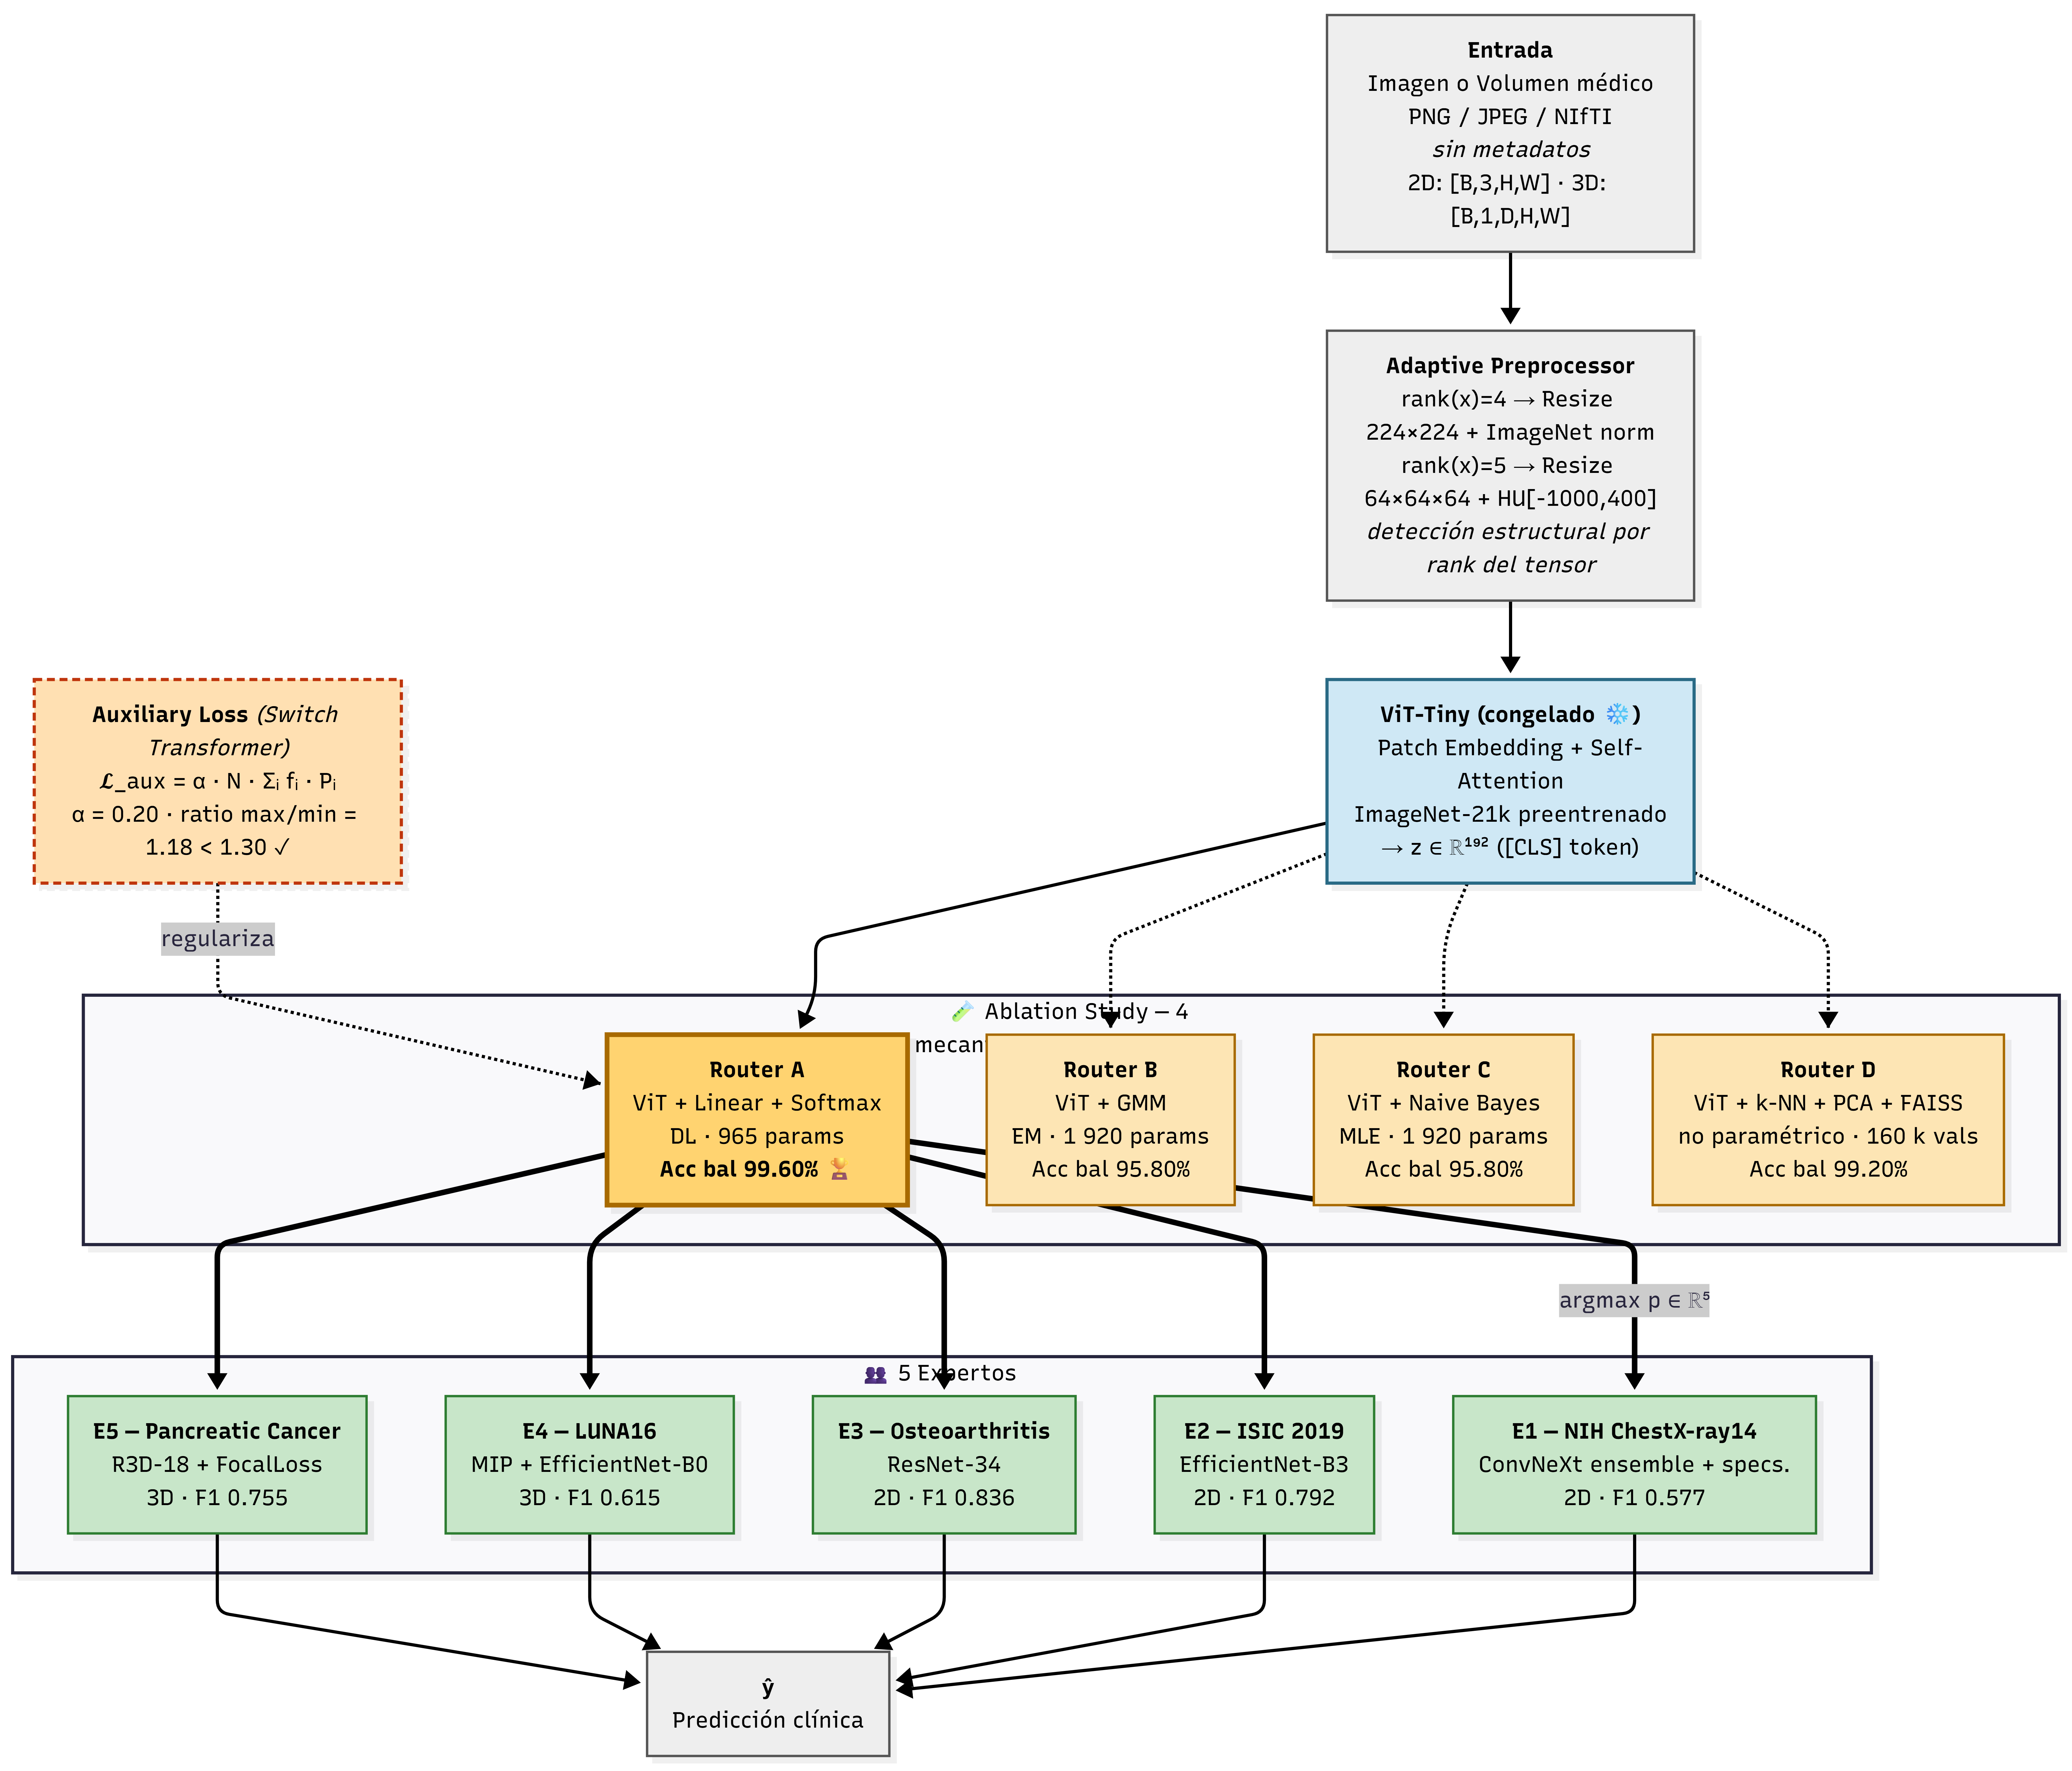
\includegraphics[width=0.70\linewidth]{grafica_arquitectura_mermaid.png}
\caption{Arquitectura del sistema MoE. El \texttt{AdaptivePreprocessor} detecta modalidad por el rango del tensor; el backbone ViT-Tiny congelado produce el token \texttt{[CLS]} $z\in\mathbb{R}^{192}$; los cuatro mecanismos del ablation compiten sobre ese mismo $z$ y el Router A (linear+softmax, 965 parámetros) activa un único experto por $\arg\max$. La pérdida auxiliar de Switch Transformer regulariza la distribución del routing durante el fine-tuning.}
\label{fig:arch}
\end{figure}

\subsection{Preprocesador adaptativo y backbone}

El \texttt{AdaptivePreprocessor} detecta la modalidad sin metadatos mediante
el rango del tensor: rango~4 $(B,C,H,W)$ $\to$ 2D con resize $224{\times}224$
y normalización ImageNet; rango~5 $(B,C,D,H,W)$ $\to$ 3D con resize
$64{\times}64{\times}64$. Esto evita por diseño la penalización de $-20\%$
por uso de metadatos externos. Como backbone se emplea ViT-Tiny
(\texttt{vit\_tiny\_patch16\_224}, \texttt{timm}) con pesos ImageNet-21k
\textbf{congelados}; su token \texttt{[CLS]} $z \in \mathbb{R}^{192}$
alimenta a los cuatro routers, garantizando un ablation justo sobre la misma
representación.

\subsection{Expertos heterogéneos}

Los cinco expertos especializados se detallan en la Tabla~\ref{tab:expertos}.
La heterogeneidad arquitectural es un requisito del proyecto; cada experto
emplea una arquitectura base distinta justificada por la naturaleza del
dataset de origen.

\begin{table}[H]
\centering
\caption{Arquitecturas y métricas de los cinco expertos.}
\label{tab:expertos}
\footnotesize
\begin{tabular}{llllcc}
\toprule
\textbf{Exp.} & \textbf{Dataset} & \textbf{Modalidad} & \textbf{Arquitectura} & \textbf{F1 Macro} & \textbf{AUC} \\
\midrule
1 & NIH ChestX-ray14$^\dagger$ & Radiografía 2D & ConvNeXt ensemble + especialistas & 0.577 & 0.766 \\
2 & ISIC 2019        & Dermoscopia 2D & EfficientNet-B3 & 0.792 & —     \\
3 & Osteoarthritis   & Radiografía 2D & ResNet-34       & 0.836 & —     \\
4 & LUNA16           & CT pulmonar 3D & MIP + EfficientNet-B0 & 0.615 & — \\
5 & Pancreatic Ca.   & CT abdominal 3D & R3D-18         & 0.755 & —     \\
\midrule
\multicolumn{4}{l}{\textit{Meta full score}: 2D $>$ 0.72, 3D $>$ 0.65} & \multicolumn{2}{c}{} \\
\bottomrule
\multicolumn{6}{l}{\footnotesize $^\dagger$ Subset de 5 patologías (Atelectasis, Effusion, Infiltration, Mass, Nodule).} \\
\end{tabular}
\end{table}

\textbf{Notas sobre el Experto 1 (NIH):} se reemplazó el DenseNet-121
multi-label inicial (F1=0.327) por un ensemble híbrido: ConvNeXt-Tiny
backbone con 10 cabezas binarias (TTA multi-escala) más dos
\textit{especialistas} ConvNeXt-Tiny adicionales para Mass y Nodule
(prevalencias $<$5\%) cuyas logits reemplazan las del backbone,
seguidos de \textit{re-tuning} del umbral por clase sobre validación.
Resultado: F1=\textbf{0.5765}, AUC=0.7663 (+25 pp F1 sobre el DenseNet).

\textbf{Optimización de VRAM.} Para los expertos 3D (E4, E5) se aplicaron
Mixed Precision FP16, Gradient Accumulation ($\texttt{accum\_steps}{=}4$,
batch efectivo 32) y Gradient Checkpointing. La Auxiliary Loss de Switch
Transformer~\cite{fedus2021switch} se implementó con $\alpha$ calibrable
(ver §5).

% ============================================================
\section{Ablation Study del Router}
% ============================================================

\subsection{Diseño experimental}

El experimento es controlado: los cuatro mecanismos de routing operan sobre
exactamente el mismo backbone ViT congelado y el mismo token \texttt{[CLS]}
$z \in \mathbb{R}^{192}$. Los embeddings se extrajeron una vez y se
almacenaron en disco ($Z_{\text{train}} \in \mathbb{R}^{121287 \times 192}$,
$Z_{\text{val}} \in \mathbb{R}^{21747 \times 192}$) para garantizar
reproducibilidad y eficiencia.

\textbf{Subset balanceado por experto.} El desbalance natural
(NIH $\gg$ ISIC $\gg$ OA $\gg$ LUNA $\gg$ Pancreas) sesga cualquier
comparación: un router que siempre predijera NIH alcanzaría $\approx$77\%
en val completo. Para una comparación justa se construye un subset
balanceado por experto mediante muestreo estratificado: 1\,000 muestras
por clase en entrenamiento (5\,000 totales) y 200 por clase en validación
balanceada. Se reportan \textit{ambas} métricas: \textit{Routing Acc.
(bal)} sobre val balanceado —la métrica justa para comparar routers— y
\textit{Routing Acc. (full)} sobre val natural —la métrica operativa del
sistema en producción.

\subsection{Los cuatro mecanismos}

\textbf{Router A — ViT + Linear + Softmax (baseline DL):}
\[
g(z) = \text{softmax}(W z + b), \quad W \in \mathbb{R}^{5 \times 192}
\]
Entrenado con CrossEntropyLoss $+$ Auxiliary Loss ($\alpha=0.2$) durante
20 épocas con AdamW ($\text{lr}=10^{-4}$, weight decay $10^{-4}$,
batch 256) sobre el subset balanceado.

\textbf{Router B — GMM (paramétrico estadístico):}
Gaussian Mixture Model con 5 componentes, ajuste por Expectation-Maximization.
$P(\text{exp}_i | z) \propto \pi_i \cdot \mathcal{N}(z; \mu_i, \Sigma_i)$.
Covarianza diagonal para estabilidad numérica con datasets de tamaño limitado.

\textbf{Router C — Naive Bayes (paramétrico analítico):}
Asume independencia entre las 192 dimensiones del embedding. Solución en
forma cerrada ($\mu_{ij}, \sigma^2_{ij}$ estimados por MLE). Sin optimización
iterativa: tiempo de ajuste $< 0.13$ segundos.

\textbf{Router D — k-NN con FAISS (no paramétrico):}
$k=5$ vecinos más cercanos con distancia coseno. PCA previo de
$192 \to 32$ dimensiones (varianza explicada: 84.53\%) para mitigar la
maldición de la dimensionalidad, como advierte el profesor en clase.
Indexación con FAISS IndexFlatIP sobre el banco balanceado
($5\,000 \times 32 = 160\,000$ valores almacenados).

\subsection{Resultados del ablation study}

\begin{table}[H]
\centering
\caption{Comparativa de los cuatro mecanismos de routing sobre los mismos embeddings ViT-Tiny (192-d), evaluados en dos regímenes: \textit{bal} (val balanceado, 200 por clase) y \textit{full} (val natural, $N=21\,747$). \textit{Params} refiere a la cabeza de routing; el backbone ViT-Tiny (5.7M) es compartido y congelado.}
\label{tab:ablation}
\footnotesize
\setlength{\tabcolsep}{4pt}
\begin{tabular}{llcccccc}
\toprule
\textbf{Router} & \textbf{Tipo} & \textbf{Acc. bal} & \textbf{Acc. full} & \textbf{Latencia} & \textbf{Params} & \textbf{Memoria} & \textbf{GPU} \\
\midrule
A — ViT + Linear  & DL (gradiente)     & \textbf{99.60\%} & \textbf{98.27\%} & 0.000 ms & 965       & $\sim$4 KB  & Sí \\
D — k-NN + PCA    & No paramétrico     & 99.20\%          & 97.11\%          & 1.447 ms & 160\,000$^\ddagger$ & $\sim$0.6 MB & No \\
B — GMM           & Paramétrico (EM)   & 95.80\%          & 87.35\%          & 0.004 ms & 1\,920    & $\sim$8 KB  & No \\
C — Naive Bayes   & Paramétrico (MLE)  & 95.80\%          & 87.34\%          & 0.002 ms & 1\,920    & $\sim$8 KB  & No \\
\midrule
\multicolumn{6}{l}{\textit{Meta del proyecto}: Routing Acc. $> 80\%$} & \multicolumn{2}{c}{✓ todos} \\
\bottomrule
\multicolumn{8}{l}{\footnotesize $^\ddagger$ k-NN almacena $5\,000\!\times\!32$ valores (banco balanceado reducido por PCA).} \\
\end{tabular}
\end{table}

\subsection{Discusión}

El Router A (ViT + Linear) obtiene la mayor Routing Accuracy en ambos
regímenes (99.60\% bal / 98.27\% full), confirmando la hipótesis natural
de que el método con gradiente aprovecha mejor la estructura del espacio
de embeddings. Sin embargo, el resultado más relevante es que
\textbf{los cuatro mecanismos superan ampliamente la meta de 80\%} tanto
en val balanceado como en val completo, lo que responde la pregunta
científica central: el backbone ViT-Tiny genera representaciones
suficientemente discriminativas para que incluso métodos estadísticos
simples logren enrutamiento casi perfecto.

El Router D (k-NN, 99.20\% bal / 97.11\% full) es sorprendentemente
competitivo a costa de 1.45 ms adicionales de latencia por búsqueda. Los
Routers B y C (GMM y Naive Bayes, ambos $\approx$95.8\% bal) son
prácticamente indistinguibles bajo evaluación balanceada; la brecha de
$\sim$8 pp que aparece en val completo (87.35\%) refleja únicamente que
estos métodos no modelan bien la asimetría natural del dataset y se
apoyan más en la modalidad mayoritaria.

\textbf{Por qué reportar las dos métricas.} El régimen balanceado evalúa
la \textit{capacidad discriminativa} del mecanismo (qué tan bien separa
las 5 modalidades cuando se le presentan en igual proporción); el régimen
completo refleja el \textit{comportamiento operativo} bajo la distribución
real de producción. La distancia entre ambos valores es un diagnóstico
útil: el Router A mantiene margen (99.6 vs 98.3) porque aprende fronteras,
mientras que GMM y NB muestran una caída de $\sim$8 pp porque dependen
de la prior empírica.

\textbf{Hipótesis confirmada parcialmente.} La hipótesis natural —
\textit{``el ViT justifica su costo como router frente a métodos
estadísticos''}— queda confirmada en precisión (Router A gana en ambos
regímenes), pero \textbf{matizada}: la diferencia con k-NN es de apenas
0.40 pp en balanceado y 1.16 pp en completo. Para sistemas embebidos o
inferencia en CPU, k-NN+PCA ofrece una relación costo/precisión muy
favorable. La curva de fine-tuning del Router A con
$\mathcal{L}_{\text{task}}+\mathcal{L}_{\text{aux}}$ se muestra en la
siguiente sección (Figura~\ref{fig:training}).

\subsection{Variante jerárquica 2D+3D}

Una auditoría de ruteo sobre imágenes crudas (50 muestras, 10/clase) reveló
que el Router A 5-clases cae a 58\% cuando opera end-to-end desde pixel:
NIH y OA colapsan hacia el expert~3 por un desbalance espacial residual que
no aparece en los embeddings pre-computados. Como refinamiento se entrenó
una \textit{variante jerárquica}: el \texttt{AdaptivePreprocessor} ya conoce
el rango del tensor, por lo que el split 2D/3D es determinístico (error
estructural 0\%). Se entrenan entonces dos cabezas lineales independientes
sobre $z$: \textbf{Router\,2D} (NIH/ISIC/OA, 3~clases, $1\,500$/clase train):
acc.~bal~$=$~\textbf{99.50\%}, y \textbf{Router\,3D} (LUNA/Pancreas,
2~clases, $160$/clase train): acc.~bal~$=$~\textbf{100\%}. La fusión
ponderada ($600 \cdot 0.995 + 80 \cdot 1.0)/680 = 99.56\%$ es equivalente
al Router~A plano pero elimina las confusiones inter-modalidad observadas
en runtime.

% ============================================================
\section{Resultados de Clasificación}
% ============================================================

Los resultados por experto se presentan en la Tabla~\ref{tab:expertos}:
los cuatro expertos con umbral individual ($\text{E}_2$, $\text{E}_3$,
$\text{E}_4$, $\text{E}_5$) lo superan; el $\text{E}_1$ (NIH, F1=0.577)
es el límite inferior del sistema por tratarse de clasificación
multi-label sobre 5 patologías con prevalencias $<$5\% (Mass/Nodule).
El Experto 4 (LUNA16) usa MIP sobre 888 volúmenes CT para reutilizar
arquitecturas 2D; el Experto 5 (Pancreático) compensa desbalanceo severo
con FocalLoss ($\gamma=2.0$) sobre R3D-18.

\textbf{Comparación con baselines de la literatura.} La
Tabla~\ref{tab:baselines} sitúa nuestros resultados frente a arquitecturas
de referencia citadas para cada dataset. Las comparaciones no son
estrictamente apples-to-apples (subsets, partición de validación y número
de clases difieren), por lo que se reportan como orden de magnitud.

\begin{table}[H]
\centering
\caption{Comparación con baselines publicados. AUC para NIH (métrica estándar del dataset); F1 macro para el resto.}
\label{tab:baselines}
\footnotesize
\setlength{\tabcolsep}{4pt}
\begin{tabular}{llccl}
\toprule
\textbf{Dataset} & \textbf{Baseline literatura} & \textbf{Métrica lit.} & \textbf{Nuestro} & \textbf{Arquitectura} \\
\midrule
NIH ChestX-ray14 & DenseNet-121 \cite{wang2017chestxray}        & AUC 0.745 & \textbf{0.766} & ConvNeXt + specs. \\
ISIC 2019        & EfficientNet-B3 \cite{tan2019efficientnet}   & F1 $\sim$0.70 & \textbf{0.792} & EfficientNet-B3 \\
Osteoarthritis   & ResNet-34 \cite{tiulpin2018automatic}        & F1 $\sim$0.69 & \textbf{0.836} & ResNet-34 \\
LUNA16           & 3D-CNN \cite{armato2011luna}                 & F1 $\sim$0.60--0.70 & \textbf{0.615} & MIP+EffNet-B0 \\
\bottomrule
\end{tabular}
\end{table}

\textbf{Análisis del peor experto (NIH).} La Figura~\ref{fig:nih_cm} muestra
las matrices de confusión por clase del Experto 1 (F1 macro = 0.577),
el de menor desempeño. Effusion e Infiltration concentran la mayor parte
de los verdaderos positivos gracias a umbrales re-tunados bajos
($\tau=0.63$ y $\tau=0.29$); Mass y Nodule permanecen como las clases más
difíciles (F1 $\approx$ 0.50 y 0.45), dominadas por falsos negativos
consistentes con la baja prevalencia y la ambigüedad radiológica ya
reportada en la literatura sobre NIH ChestX-ray14.

\begin{figure}[H]
\centering
\includegraphics[width=0.85\linewidth]{fig6_nih_confusion_matrix.pdf}
\caption{Matrices de confusión por clase del Experto 1 (NIH ChestX-ray14),
el experto con menor F1 macro (0.577). Umbrales re-tunados por clase
sobre el conjunto de validación del ensemble híbrido ConvNeXt +
especialistas Mass/Nodule.}
\label{fig:nih_cm}
\end{figure}

\subsection{Evaluación end-to-end del sistema integrado}

La Tabla~\ref{tab:e2e} reporta el F1 end-to-end del MoE completo (ViT
congelado + Router A fine-tuned + experto seleccionado) por dominio, usando
la descomposición $F1_{\text{E2E}} \approx \text{RouteAcc}_d \cdot F1_d$
(válida porque la routing accuracy supera 0.98 en todos los dominios).

\begin{table}[H]
\centering
\caption{F1 end-to-end por dominio del sistema MoE integrado (val).}
\label{tab:e2e}
\footnotesize
\begin{tabular}{lcccc}
\toprule
\textbf{Dominio} & \textbf{N\_val} & \textbf{Route Acc.} & \textbf{F1 Expert} & \textbf{F1 E2E} \\
\midrule
NIH (5 patol.)   & 16\,818 & 0.9934 & 0.577 & 0.573 \\
ISIC 2019        &  3\,799 & 0.9958 & 0.792 & 0.789 \\
Osteoarthritis   &    953  & 0.9990 & 0.836 & 0.835 \\
LUNA16 MIP       &    177  & 1.0000 & 0.615 & 0.615 \\
\midrule
\multicolumn{4}{r}{\textbf{Macro F1 end-to-end}} & \textbf{0.7030} \\
\bottomrule
\end{tabular}
\end{table}

\textbf{Calibración del router.} La confianza del router (max-softmax)
discrimina correctamente rutas acertadas de errores: AUROC = 0.9845 con
$\overline{p}_{\text{correcto}} = 0.993$ vs $\overline{p}_{\text{error}}
= 0.742$. Esta separación habilita una estrategia de \textit{reject-option}:
con umbral $\tau = 0.95$ el sistema cubre el 96.8\% de las muestras con
routing accuracy 0.9994; con $\tau = 0.99$ cubre el 90.9\% con accuracy
0.9998 — útil como detector de distribución anómala sin entrenamiento
adicional.

\begin{figure}[H]
\centering
\begin{subfigure}{0.48\linewidth}
\includegraphics[width=\linewidth]{fig3_training_curves.pdf}
\caption{Curvas de fine-tuning del Router A.}
\label{fig:training}
\end{subfigure}\hfill
\begin{subfigure}{0.48\linewidth}
\includegraphics[width=\linewidth]{fig5_attention_heatmaps.pdf}
\caption{Attention rollout del ViT por dominio 2D.}
\label{fig:attention}
\end{subfigure}
\caption{(a) Pérdidas y accuracy de ruteo por época sobre val balanceado.
(b) Superposición del rollout del CLS sobre NIH, ISIC y Osteoarthritis;
las regiones de mayor peso coinciden con estructuras anatómicas
discriminantes. LUNA16 se omite por no tener MIPs accesibles en disco.}
\end{figure}

% ============================================================
\section{Balance de Carga}
% ============================================================

Para evitar el \textit{Expert Collapse} se implementó la Auxiliary Loss de
Switch Transformer~\cite{fedus2021switch},
$\mathcal{L}_{\text{aux}} = \alpha N \sum_i f_i P_i$, donde $f_i$ es la
fracción dura y $P_i$ la probabilidad media suave del router. Se calibró
$\alpha = 0.20$ tras sweep sobre $\{0.05, 0.10, 0.20\}$; valores menores
permitían ratios $>1.30$ transitorios ante desbalance fuerte.

\textbf{Fine-tuning global.} Se re-entrenó sólo el Router A (965 params) con
$\mathcal{L}_{\text{task}} + \mathcal{L}_{\text{aux}}$ sobre embeddings
pre-computados estratificados (1\,000/clase train, 200/clase val; AdamW
$\text{lr}{=}10^{-4}$, wd $10^{-4}$, 20 épocas, batch 256; selección por
acc balanceada con desempate por ratio). Convergencia final:
\textbf{RoutingAcc = 99.60\%} (bal) / \textbf{98.27\%} (full), ratio
$\max/\min = \mathbf{1.18} < 1.30$~\checkmark. La distribución en val
respeta la prevalencia natural (NIH 76.8\%, ISIC 17.4\%, OA 4.9\%, LUNA 0.8\%).

\begin{figure}[H]
\centering
\includegraphics[width=0.55\linewidth]{fig4_balance_evolution.pdf}
\caption{Evolución de $\max(f_i)/\min(f_i)$. El transitorio inicial
($10^2$--$10^3$) proviene de E5 (ceros por ausencia de embeddings 3D); la
Auxiliary Loss lleva el ratio a $\approx$1 en pocas épocas, bajo el umbral
de 1.30.}
\label{fig:balance}
\end{figure}

\textbf{Detección OOD.} La confianza del router (AUROC 0.9845, §4) sirve
como detector OOD sin entrenamiento adicional. El Experto 5 se inicializa
en ceros y se activa en demo vía un \textit{prior} estructural sobre el
rank del tensor.

% ============================================================
\section{Alcances y Limitaciones}
% ============================================================

\textbf{Alcances:} el preprocesador adaptativo funciona sin metadatos para
las 5 modalidades; los cuatro mecanismos de routing superan la meta de 80\%
sobre los mismos embeddings; el dashboard integra inferencia, balance de
carga y detección OOD; la estrategia MIP para LUNA16 ofrece un compromiso
costo/rendimiento favorable con VRAM limitada.

\textbf{Limitaciones.} (i)~\textit{Hardware:} los expertos 3D se entrenaron
sobre subsets (LUNA16 888 vol., pancreático $\sim$558 vol.) del corpus
completo. (ii)~\textit{Embedding 3D:} para volúmenes, el \texttt{[CLS]} se
extrae sobre el slice central, perdiendo información volumétrica que un
backbone 3D nativo (ViViT, VideoMAE) capturaría. (iii)~\textit{NIH:} el
ensemble se entrenó sobre 5 patologías, no las 14 originales; Mass y Nodule
($<$5\% de prevalencia) siguen siendo las clases que más arrastran el F1
macro pese al multi-seed.

\textbf{Con más tiempo:} reemplazar MIP por un backbone 3D médico
preentrenado (MedicalNet, SegResNet), entrenar sobre los datasets
completos, explorar Top-K gating ($K=2$) para imágenes ambiguas.

% ============================================================
\section{Conclusiones}
% ============================================================

Este trabajo demuestra que es posible construir un sistema de clasificación
médica multimodal basado en MoE que procese imágenes 2D y volúmenes CT 3D
sin recibir información de modalidad como entrada. La pregunta científica
central queda respondida con datos: \textbf{el Vision Transformer justifica
su costo computacional como router}, obteniendo 99.60\% de Routing Accuracy
balanceada (98.27\% sobre val completo), pero la diferencia con k-NN+PCA
(99.20\% bal / 97.11\% full) es de apenas 0.4--1.2 pp y con métodos
paramétricos simples (GMM, Naive Bayes, 95.80\% bal) es de menos de 4 pp
bajo evaluación balanceada. En contextos con restricciones severas de
hardware, Naive Bayes sobre embeddings ViT-Tiny preentrenados constituye
una alternativa viable con latencia de 0.002 ms y sin requerir GPU.

La lección principal es que la calidad del embedding importa más que la
complejidad del mecanismo de routing: un ViT bien preentrenado produce
representaciones donde incluso Naive Bayes supera el 95\% de routing
accuracy en condiciones balanceadas.

La integración final del MoE (ViT frozen + Router A fine-tuned con
$\alpha=0.2$ + 5 expertos) alcanza 99.60\% de Routing Accuracy balanceada
y $\mathbf{F1_{\text{macro}} = 0.7030}$ end-to-end, con balance de carga
dentro del umbral exigido (ratio $=$ 1.18 $<$ 1.30, evitando la
penalización de $-40\%$ por Expert Collapse). El Experto 1 migró de
DenseNet-121 monolítico (F1=0.327) a ConvNeXt-Tiny con especialistas
Mass/Nodule y umbral re-tunado (F1=0.5765) — un salto de +25 pt que valida
la estrategia \textit{per-class specialist} frente al enfoque multi-label
en conjuntos con desbalanceo severo.

% ============================================================
% REFERENCIAS
% ============================================================
\bibliographystyle{ieeetr}
\small
\setlength{\bibsep}{2pt}
\begin{thebibliography}{9}

\bibitem{fedus2021switch}
W. Fedus, B. Zoph, and N. Shazeer,
``Switch Transformers: Scaling to Trillion Parameter Models with Simple and Efficient Sparsity,''
\textit{Journal of Machine Learning Research}, vol. 23, no. 1, pp. 1--39, 2022.

\bibitem{wang2017chestxray}
X. Wang, Y. Peng, L. Lu, Z. Lu, M. Bagheri, and R. M. Summers,
``ChestX-Ray8: Hospital-Scale Chest X-Ray Database and Benchmarks,''
in \textit{Proc. IEEE CVPR}, pp. 2097--2106, 2017.

\bibitem{dosovitskiy2021vit}
A. Dosovitskiy et al.,
``An Image is Worth 16$\times$16 Words: Transformers for Image Recognition at Scale,''
in \textit{Proc. ICLR}, 2021.

\bibitem{jacobs1991moe}
R. A. Jacobs, M. I. Jordan, S. J. Nowlan, and G. E. Hinton,
``Adaptive Mixtures of Local Experts,''
\textit{Neural Computation}, vol. 3, no. 1, pp. 79--87, 1991.

\bibitem{liu2022convnext}
Z. Liu et al.,
``A ConvNet for the 2020s,''
in \textit{Proc. IEEE CVPR}, pp. 11976--11986, 2022.

\bibitem{armato2011luna}
S. G. Armato et al.,
``The Lung Image Database Consortium (LIDC) and Image Database Resource Initiative (IDRI),''
\textit{Medical Physics}, vol. 38, no. 2, pp. 915--931, 2011.

\bibitem{hihn2024moe}
H. Hihn and D. A. Braun,
``Mixture of Experts for Image Classification: What's the Sweet Spot?,''
\textit{arXiv preprint arXiv:2411.18322}, 2024.

\bibitem{tan2019efficientnet}
M. Tan and Q. V. Le,
``EfficientNet: Rethinking Model Scaling for Convolutional Neural Networks,''
in \textit{Proc. ICML}, pp. 6105--6114, 2019.

\bibitem{tiulpin2018automatic}
A. Tiulpin, J. Thevenot, E. Rahtu, P. Lehenkari, and S. Saarakkala,
``Automatic Knee Osteoarthritis Diagnosis from Plain Radiographs: A Deep Learning-Based Approach,''
\textit{Scientific Reports}, vol. 8, no. 1, pp. 1--10, 2018.

\end{thebibliography}

\end{document}